\documentclass[article,shortnames]{jss}
\usepackage[utf8]{inputenc}

\providecommand{\tightlist}{%
  \setlength{\itemsep}{0pt}\setlength{\parskip}{0pt}}

\author{
Victor Maus\\University of Münster\\INPE, IIASA \And Gilberto Câmara\\INPE\\University of Münster \And Marius Appel\\University of Münster\\ \And Edzer Pebesma\\University of Münster\\
}
\title{\pkg{dtwSat}: Time-Weighted Dynamic Time Warping for Satellite Image
Time Series Analysis in \proglang{R}}
\Keywords{dynamic programming, MODIS time series, land cover changes, crop monitoring}

\Abstract{
The opening of large archives of satellite data such as LANDSAT, MODIS
and the SENTINELs has given researchers unprecedented access to data,
allowing them to better quantify and understand local and global land
change. The need to analyse such large data sets has lead to the
development of automated and semi-automated methods for satellite image
time series analysis. However, few of the proposed methods for remote
sensing time series analysis are available as open source software. In
this paper we present the \proglang{R} package \pkg{dtwSat}. This
package provides an implementation of the Time-Weighted Dynamic Time
Warping method for land cover mapping using sequence of multi-band
satellite images. Methods based on dynamic time warping are flexible to
handle irregular sampling and out-of-phase time series, and they have
achieved significant results in time series analysis. \pkg{dtwSat} is
available from the Comprehensive R Archive Network and contributes to
making methods for satellite time series analysis available to a larger
audience. The package supports the full cycle of land cover
classification using image time series, ranging from selecting temporal
patterns to visualising and assessing the results.
}

\Plainauthor{Victor Maus, Gilberto Câmara, Marius Appel, Edzer Pebesma}
\Plaintitle{dtwSat: Time-Weighted Dynamic Time Warping for Satellite Image Time
Series Analysis in R}
\Shorttitle{\pkg{dtwSat}: Time-Weighted Dynamic Time Warping}
\Plainkeywords{dynamic programming, MODIS time series, land cover changes, crop monitoring}

%% publication information
%% \Volume{50}
%% \Issue{9}
%% \Month{June}
%% \Year{2012}
\Submitdate{}
%% \Acceptdate{2012-06-04}

\Address{
    Victor Maus\\
%%  University of Münster\\
  Ecosystems Services and Management Program\newline International
  Institute for Applied Systems Analysis\newline Schlossplatz
  1\newline A-2361 Laxenburg, Austria\\
  E-mail: \href{mailto:vwmaus1@gmail.com}{\nolinkurl{vwmaus1@gmail.com}}\\
  URL: \url{www.iiasa.ac.at/staff/maus}\\~\\
        }

\usepackage{amsmath} \usepackage{array} \usepackage{caption}
\usepackage{subcaption} \usepackage{float} \usepackage{microtype}
\setlength{\tabcolsep}{4pt} \usepackage{xcolor}
\usepackage[printwatermark]{xwatermark}

\begin{document}

\newwatermark[allpages,angle=45,scale=1.5,xpos=0,ypos=0]{Conditionally accepted}
\sloppy

\section{Introduction}\label{introduction}

Remote sensing images are the most widely used data source for measuring
land use and land cover change (LUCC). In many areas, remote sensing
images are the only data available for this purpose
\citep{Lambin:2006, Fritz:2013}. Recently, the opening of large archives
of satellite data such as LANDSAT, MODIS and the SENTINELs has given
researchers unprecedented access to data, allowing them to better
quantify and understand local and global land change. The need to
analyse such large data sets has lead to the development of automated
and semi-automated methods for satellite image time series analysis.
These methods include multi-image compositing \citep{Griffiths:2013},
detecting forest disturbance and recovery
\citep{Kennedy:2010, Zhu:2012, DeVries:2015}, crop classification
\citep{Xiao:2005, Wardlow:2007, Petitjean:2012, Maus:2016}, planted
forest mapping \citep{Maire:2014}, crop expansion and intensification
\citep{Galford:2008, Sakamoto:2009}, detecting trend and seasonal
changes
\citep{Lunetta:2006, Verbesselt:2010, Verbesselt:2010a, Verbesselt:2012},
and extracting seasonality metrics from satellite time series
\citep{Jonsson:2002, Jonsson:2004}. Given the open availability of large
image data sets, the Earth Observation community would get much benefit
from methods that are openly available, reproducible and comparable.
However, few of the proposed methods for remote sensing time series
analysis are available as open source software, the main exception being
the BFAST and BFAST-monitor algorithms for change detection
\citep{Verbesselt:2010, Verbesselt:2010a}. This paper is a contribution
to making methods for satellite time series analysis available to a
larger audience.

In this paper we describe the \pkg{dtwSat} package, written in
\proglang{R} \citep{R:2015} and \proglang{Fortran} programming
languages, and available from the Comprehensive R Archive Network at
\url{http://CRAN.R-project.org/package=dtwSat}. The package provides an
implementation of Time-Weighted Dynamic Time Warping (TWDTW)
\citep{Maus:2016} for satellite image time series analysis.

The TWDTW method is an adaptation of the well-known dynamic time warping
(DTW) method for time series analysis
\citep{Velichko:1970, Sakoe:1971, Sakoe:1978, Rabiner:1993, Berndt:1994, Keogh:2005, Muller:2007}
for land cover classification. The standard DTW compares a temporal
signature of a known event (\emph{e.g.}, a person's speech) with an
unknown time series. It finds all possible alignments between two time
series and provides a dissimilarity measure \citep{Rabiner:1993}. In
contrast to standard DTW, the TWDTW method is sensitive to seasonal
changes of natural and cultivated vegetation types. It also considers
inter-annual climatic and seasonal variability. In a tropical forest
area, the method has achieved a high accuracy for mapping classes of
single cropping, double cropping, forest, and pasture \citep{Maus:2016}.

We chose \proglang{R} because it is an open source software that offers
a large number of reliable packages. The \pkg{dtwSat} package builds
upon on a number of graphical and statistical tools in \proglang{R}:
\pkg{dtw} \citep{Giorgino:2009}, \pkg{proxy} \citep{Meyer:2015},
\pkg{zoo} \citep{Zeileis:2005}, \pkg{mgcv}
\citep{Wood:2000, Wood:2003, Wood:2004, Wood:2006, Wood:2011}, \pkg{sp}
\citep{Pebesma:2005, Bivand:2013}, \pkg{raster} \citep{Hijmans:2015},
\pkg{caret} \citep{Kuhn:2016}, and \pkg{ggplot2} \citep{Wickham:2009}.
Other \proglang{R} packages that are related and useful for remote
sensing and land cover analysis include \pkg{landsat}
\citep{Goslee:2011}, \pkg{rgdal} \citep{Bivand:2015}, \pkg{spacetime}
\citep{Pebesma:2012, Bivand:2013}, \pkg{bfast}
\citep{Verbesselt:2010, Verbesselt:2010a}, \pkg{bfastmonitor}
\citep{Verbesselt:2011}, \pkg{bfastSpatial} \citep{Dutrieux:2014},
\pkg{MODISTools} \citep{Tuck:2014}, \pkg{maptools} \citep{Bivand:2015},
and \pkg{lucc} \citep{Moulds:2015}. Using existing packages as building
blocks, software developers in \proglang{R} save a lot of time and can
concentrate on their intended goals.

There is already an \proglang{R} package that implements the standard
DTW method for time series analysis: the \pkg{dtw} package
\citep{Giorgino:2009}. In the \pkg{dtwSat} package, we focus on the
specific case of satellite image time series analysis. The analysis
method implemented in \pkg{dtwSat} package extends that of the \pkg{dtw}
package; it adjusts the standard DTW method to account for the
seasonality of different types of land cover. Our aim is to support the
full cycle of land cover classification, from selecting sample patterns
to visualising and assessing the final result.

This paper focuses on the motivation and guidance for using the TWDTW
method for remote sensing applications. The full description of the
method is available in a paper published by the lead author
\citep{Maus:2016}. In what follows, the
\autoref{the-time-weighted-dynamic-time-warping-method} describes the
application of TWDTW \citep{Maus:2016} for satellite time series
analysis. The \autoref{dtwsat-package-overview} gives an overview of the
\pkg{dtwSat} package. Then, \autoref{classifying-a-time-series} focuses
on the analysis of a single time series and shows some visualisation
methods. We then present an example of a complete land cover change
analysis for a study area in Mato Grosso, Brazil in
\autoref{producing-a-land-cover-map}.

\section{The Time-Weighted Dynamic Time Warping
method}\label{the-time-weighted-dynamic-time-warping-method}

In this section, we describe the Time-Weighted Dynamic Time Warping
(TWDTW) algorithm in general terms. For a detailed technical
explanation, refer to \citet{Maus:2016}. TWDTW is time-constrained
version of the Dynamic Time Warping (DTW) algorithm. Although the
standard DTW method is good for shape matching \citep{Keogh:2005}, it is
not suited \emph{per se} for satellite image time series analysis, since
it disregards the temporal range when finding the best matches between
two time series \citep{Maus:2016}. When using image time series for land
cover classification, one needs to balance between shape matching and
temporal alignment, since each land cover class has a distinct
phenological cycle associated with the vegetation
\citep[\citet{Zhang:2003}]{Reed:1994}. For example, soybeans and maize
cycles range from 90 to 120 days, whereas sugar-cane has a 360 to 720
days cycle. A time series with cycle larger than 180 days is unlikely to
come from soybeans or maize. For this reason, \citet{Maus:2016} include
a time constraint in DTW to account for seasonality. The resulting
method is capable of distinguishing different land cover classes.

The inputs to TWDTW are: (a) a set of time series of known temporal
patterns (\emph{e.g.}, phenological cycles of land cover classes); (b)
an unclassified long-term satellite image time series. For each temporal
pattern, the algorithm finds all matching subintervals in the long-term
time series, providing a dissimilarity measure (cf.
\autoref{fig:twdtw-example}). The result of the algorithm is a set of
subintervals, each associated with a pattern and with a dissimilarity
measure. We then break the unclassified time series in periods according
to our needs (\emph{e.g.}, yearly, seasonality, monthly). For each
period, we consider all matching subintervals that intersect with it,
and classify them based on the land cover class of the best matching
subinterval. In this way, the long-term satellite time series is divided
in periods, and each period is assigned a land cover class.

\begin{CodeChunk}
\begin{figure}[h]

{\centering 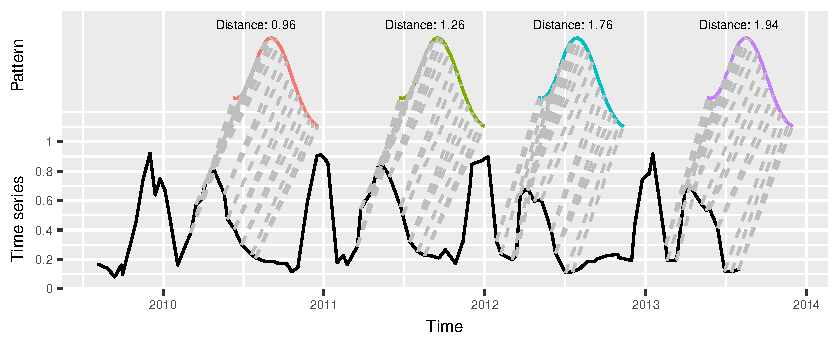
\includegraphics{applying_twdtw_files/figure-latex/twdtw-example-1} 

}

\caption[Matches of the known temporal pattern to subintervals of the long-term time series]{Matches of the known temporal pattern to subintervals of the long-term time series. The solid black line is the long-term time series, the colored lines are the different matches of the same pattern ordered by TWDTW dissimilarity measure, and the gray dashed lines are the matching points.}\label{fig:twdtw-example}
\end{figure}
\end{CodeChunk}

To use TWDTW for land cover classification, we need the following data
sets:

\begin{itemize}
\item
  A set of remote sensing time series for the study area. For example, a
  tile of a MODIS MOD13Q1 image consists of 4800 x 4800 pixels, covering
  an area of 10 degrees x 10 degrees at the Equator \citep{Friedl:2010}.
  A 15-year (2000-2015) MODIS MOD13Q1 set time series has 23 images per
  year, with a total of 23 million time series, each with 346 samples.
\item
  A set of time series with land cover information, called
  \emph{temporal patterns}. Typically, each time series is short and
  covers one phenological cycle of one land cover type. Examples would
  be a time series of a soybean crop, or one that describes a mature
  tropical forest. These temporal patterns can be extracted from the
  remote sensing image data, if the user knows their spatial and
  temporal location.
\item
  A set of ground truth points, with spatial and temporal information
  and land cover classification. These \emph{ground truth} points are
  used for validation and accuracy assessment.
\end{itemize}

Based on the information provided by the user about the images to be
analysed, our method maps them to a three-dimensional (3-D) array in
space-time (\autoref{fig:3-D-array}). This array can have multiple
attributes, such as the satellite bands (\emph{e.g.}, ``red'', ``nir'',
and ``blue''), and derived indices (\emph{e.g.}, ``NDVI'', ``EVI'', and
``EVI2''). This way, each pixel location is associated to a sequence of
measurements, building a satellite image time series.
\autoref{fig:3-D-array} shows an example of ``EVI'' time series for a
location in the Brazilian Amazon from 2000 to 2008. In the first two
years, the area was covered by forest that was cut in 2002. The area was
then used for cattle raising (pasture) for three years, and then for
crop production from 2006 to 2008. Satellite image time series are thus
useful to describe the dynamics of the landscape and the land use
trajectories.

\begin{figure}[!h]
\begin{center} 
  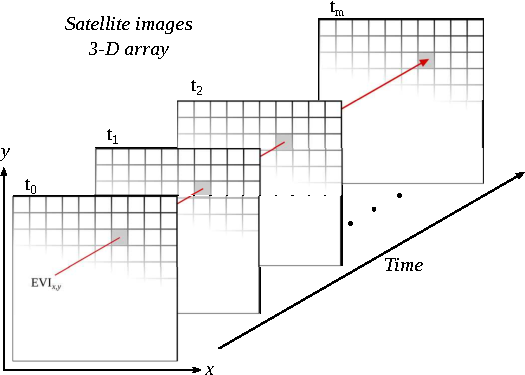
\includegraphics[width=.45\textwidth]{./images_array.pdf}
  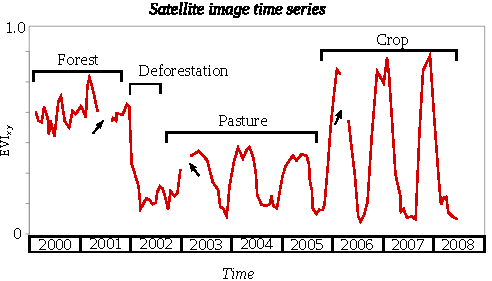
\includegraphics[width=.45\textwidth]{./images_ts.pdf}
\end{center}
\caption{A 3-dimensional array of satellite images (left), an enhanced vegetation index (EVI) time series at the pixel location $(x,y)$ (right). The arrows indicate gaps in the time series. Adapted from \citet{Maus:2016}.}
\label{fig:3-D-array}
\end{figure}

\section{dtwSat package overview}\label{dtwsat-package-overview}

\pkg{dtwSat} provides a set of functions for land cover change analysis
using satellite image time series. This includes functions to build
temporal patterns for land cover types, apply the TWDTW analysis using
different weighting functions, visualise the results in a graphical
interface, produce land cover maps, and create spatiotemporal plots for
land changes. Therefore, \pkg{dtwSat} gives an end-to-end solution for
satellite time series analysis, which users can make a complete land
change analysis.

For the \pkg{dtwSat} package, the user should provide the following
inputs:

\begin{itemize}
\item
  A set of time ordered satellite images, all with the same spatial
  extent. The user should also inform the date of each image. In
  \proglang{R} the images should use the \code{RasterBrick} or
  \code{RasterStack} class of the \pkg{raster} package.
\item
  A list of temporal patterns, each associated to a time series in
  \pkg{zoo} format.
\item
  A list of known ground truth points, each with spatial and temporal
  information, in a format readable in \proglang{R}, such as CSV or
  shapefile.
\end{itemize}

The \pkg{dtwSat} package organizes the data in three \code{S4} classes
of objects: \code{twdtwTimeSeries}, \code{twdtwMatches}, and
\code{twdtwRaster}. To store time series we use the class
\code{twdtwTimeSeries}. The objects of class \code{twdtwTimeSeries} have
two slots; the slot called \code{timeseries} has a list of \code{zoo}
objects; and the slot called \code{labels} stores the labels of the time
series. The class \code{twdtwMatches} has 3 slots to store inputs and
results of the TWDTW analysis. The slots called \code{timeseries} and
\code{patterns} are objects of the class \code{twdtwTimeSeries} with the
unclassified long-term time series and the temporal patterns,
respectively. A third slot called \code{alignments} has a \code{list}
with detailed information about the matches between the patterns and the
unclassified long-term time series. The classes \code{twdtwTimeSeries}
and \code{twdtwMatches} are used to analyse lists of time series.

The class \code{twdtwRaster} is used for satellite image time series.
This class can store either unclassified raster time series with the
satellite raw data, the results of the TWDTW analyis, or a classified
raster time series. In both cases, the objects of class
\code{twdtwRaster} have five slots. The slot called \code{timeseries} is
a list of \code{RasterBrick} or \code{RasterStack} objects with time
ordered satellite images (all with the same temporal and spatial
extents); the slot called \code{timeline} is a vector of class
\code{Date} with dates of the satellite images; the slot called
\code{layers} has the names of satellite bands; the slot called
\code{levels} has levels for the raster values; and the slot called
\code{labels} has labels for the raster values. This class builds upon
the \proglang{R} package \pkg{raster} to build a multi-attribute 3-D
raster in space-time, allowing for multi-band satellite image time
series analysis.

\section{Classifying a time series}\label{classifying-a-time-series}

This section describes how to classify one time series, using examples
that come with the \pkg{dtwSat} package. We will show how to match three
temporal patterns (``soybean'', ``cotton'', and ``maize'') to
subintervals of a long-term satellite image time series. These time
series have been extracted from a set of MODIS MOD13Q1
\citep{Friedl:2010} images and include the vegetation indices ``ndvi'',
``evi'', and the original bands ``nir'', ``red'', ``blue'', and ``mir''.
In this example, the classification of crop types for the long-term time
series is known.

\subsection{Input data}\label{input-data}

The inputs for the next examples are time series in \pkg{zoo} format.
The first is an object of class \code{zoo} with a long-term time series,
referred to as \code{MOD13Q1.ts}, and the second is a \code{list} of
time series of class \code{zoo} with the temporal patterns of
``soybean'', ``cotton'', and ``maize'', referred to as
\code{MOD13Q1.patterns.list}.

From \code{zoo} objects we construct time series of class
\code{twdtwTimeSeries}, for which we have a set of visualization and
analysis methods implemented in the \pkg{dtwSat} package. The code below
builds two objects of class \code{twdtwTimeSeries}. The first has the
long-term time series and second has the temporal patterns. We use the
plot method types \code{timeseries} and \code{patterns} to shown the
objects \code{ts} in \autoref{fig:example-timeseries} and
\code{MOD13Q1.ts} in \autoref{fig:temporal-patterns-soy-cot-mai},
respectively. This plot method uses \code{ggplot} syntax.

\begin{CodeChunk}
\begin{CodeInput}
library(dtwSat)
names(MOD13Q1.patterns.list)
\end{CodeInput}
\begin{CodeOutput}
[1] "Soybean" "Cotton"  "Maize"  
\end{CodeOutput}
\begin{CodeInput}
head(MOD13Q1.ts, n = 2)
\end{CodeInput}
\begin{CodeOutput}
             ndvi    evi    red    nir   blue    mir
2009-08-05 0.3169 0.1687 0.1167 0.2250 0.0427 0.2193
2009-08-28 0.2609 0.1385 0.1168 0.1993 0.0548 0.2657
\end{CodeOutput}
\end{CodeChunk}\begin{CodeChunk}
\begin{CodeInput}
ts = twdtwTimeSeries(MOD13Q1.ts, labels="Time series")
patterns_ts = twdtwTimeSeries(MOD13Q1.patterns.list)
patterns_ts
\end{CodeInput}
\begin{CodeOutput}
An object of class "twdtwTimeSeries"
Slot "timeseries" length: 3 
Slot "labels": [1] "Soybean" "Cotton"  "Maize"  
\end{CodeOutput}
\end{CodeChunk}

\begin{CodeChunk}
\begin{CodeInput}
plot(ts, type = "timeseries") + 
  annotate(geom = "text", x = MOD13Q1.ts.labels$from+90, y = 0.98, 
  label = MOD13Q1.ts.labels$label, size = 2)
\end{CodeInput}
\begin{figure}[!h]

{\centering 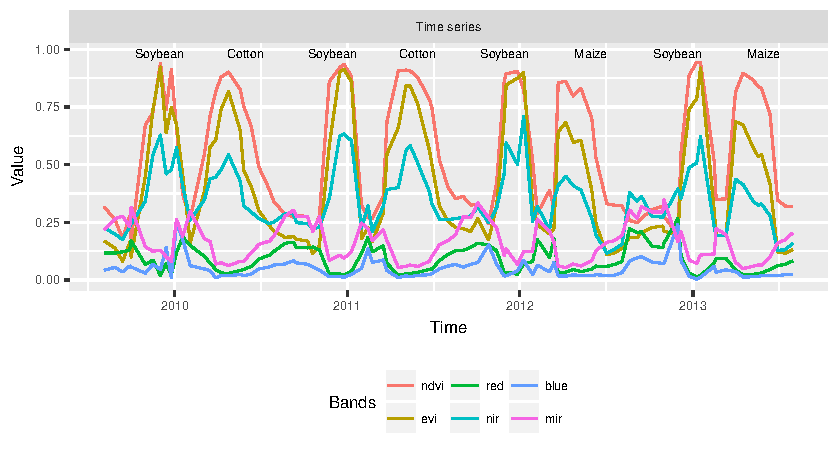
\includegraphics{applying_twdtw_files/figure-latex/example-timeseries-1} 

}

\caption{Example of time series based on MODIS product MOD13Q1 \citep{Friedl:2010}. The labels of the phenological cycle are shown in the plot.}\label{fig:example-timeseries}
\end{figure}
\end{CodeChunk}\begin{CodeChunk}
\begin{CodeInput}
plot(patterns_ts, type = "patterns")
\end{CodeInput}
\begin{figure}[!h]

{\centering 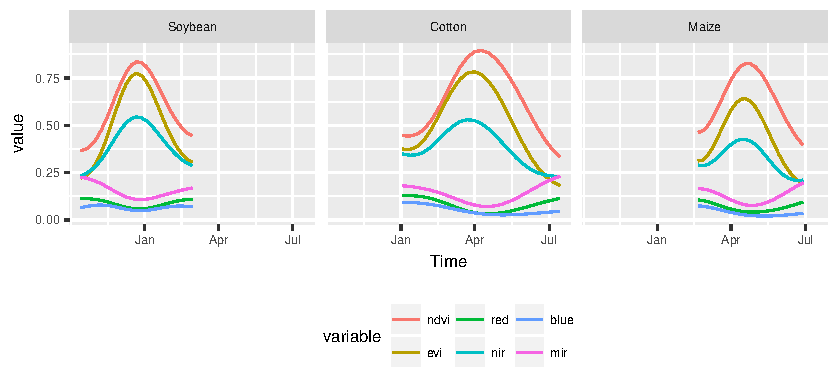
\includegraphics{applying_twdtw_files/figure-latex/temporal-patterns-soy-cot-mai-1} 

}

\caption{Temporal patterns of soybean, cotton, and maize based on MODIS product MOD13Q1 \citep{Friedl:2010}.}\label{fig:temporal-patterns-soy-cot-mai}
\end{figure}
\end{CodeChunk}

TWDTW uses both amplitude and phase information to classify the
phenological cycles in the long-term time series. The differences in the
amplitude and phase of the cycles are more clear when we observe the EVI
signal in Figures 3 and 4. The EVI peak of the ``soybean'' time series
has a similar amplitude as that of ``cotton''. However, the ``soybean''
series peaks in late December while the ``cotton'' series peaks in early
April. The EVI peak of the ``maize'' time series is at the same period
as the peak of ``cotton''. However, the ``maize'' time series has
smaller amplitude than the ``cotton'' one. Therefore, combining shape
and time information we can improve the time series classification.

\subsection{Detection of time series patterns with
TWDTW}\label{detection-of-time-series-patterns-with-twdtw}

Each subinterval of the long-term time series in \code{ts} has a known
phenological cycle. We will now compare the known information with the
result of the TWDTW algorithm. We use the function \code{twdtwApply}
that returns an \proglang{R} object of class \code{twdtwMatches} with
all matches of each temporal pattern in the time series.

\begin{CodeChunk}
\begin{CodeInput}
log_weight = logisticWeight(alpha = -0.1, beta = 100)
matches = 
  twdtwApply(x = ts, y = patterns_ts, weight.fun = log_weight, keep=TRUE)
slotNames(matches)
\end{CodeInput}
\begin{CodeOutput}
[1] "timeseries" "patterns"   "alignments"
\end{CodeOutput}
\begin{CodeInput}
show(matches)
\end{CodeInput}
\begin{CodeOutput}
An object of class "twdtwMatches"
Number of time series: 1 
Number of Alignments: 27 
Patterns labels: Soybean Cotton Maize 
\end{CodeOutput}
\end{CodeChunk}

To retrieve the complete information of the matches we set
\code{keep=TRUE}. We need this information for the plot methods of the
class \code{twdtwMatches}. The argument \code{weight.fun} defines the
time-weight to the dynamic time warping analysis \citep{Maus:2016}. By
default the time-weight is zero, meaning that the function will run a
standard dynamic time warping analysis. The arguments \code{x} and
\code{y} are objects of class \code{twdtwTimeSeries} with the
unclassified long-term time series and the temporal patterns,
respectively. To perform the alignment between the time series the
default TWDTW recursion has a symmetric step (for more details and other
recursion options see \code{?stepPattern}). \citet{Giorgino:2009}
provides a detaild discussion on the recursion steps and other step
patterns. For further details and other arguments of the TWDTW analysis
see \code{?twdtwApply}.

In our example we use a logistic weight function for the temporal
constraint of the TWDTW algorithm. This function is defined by
\code{logisticWeight}. The \pkg{dtwSat} package provides two in-built
functions: \code{linearWeight} and \code{logisticWeight}. The
\code{linearWeight} function with slope \code{a} and intercept \code{b}
is given by \[
    \omega = a \cdot g(t_1,t_2) + b,
    \label{eq:lineartw}
\] and the \code{logisticWeight} with midpoint \code{beta}, and
steepness \code{alpha}, given by \[
    \omega = \frac{1}{1 + e^{-\alpha(g(t_1,t_2)-\beta)} }.
    \label{eq:nonlineartw}
\] The function \(g\) is the absolute difference in days between two
dates, \(t_1\) and \(t_2\). The aim of these functions is to control the
time warp, e.g.~a ``large time warp'' is needed to match a point of the
temporal pattern whose original date is January 1 to a point of the
long-term time series whose date is July 1, on the other hand to match
January 1 to December 15 has a ``small time warp''. If there is a large
seasonal difference between the pattern and its matching point in time
series, an extra cost is added to the DTW distance measure. This
constraint controls the time warping and makes the time series alignment
dependent on the seasons. This is especially useful for detecting
temporary crops and for distinguishing pasture from agriculture. The
linear function creates a strong time constraint even for small time
differences, including small time warps. The logistic function has a low
weight for small time warps and significant costs for bigger time warps,
cf. \autoref{fig:logist-time-weight}. In our previous studies
\citep{Maus:2016} the logistic-weight had better results than the
linear-weight for land cover classification. Users can define different
weight functions as temporal constraints in the argument
\code{weight.fun} of the function \code{twdtwApply}.

\begin{CodeChunk}
\begin{figure}[!h]

{\centering 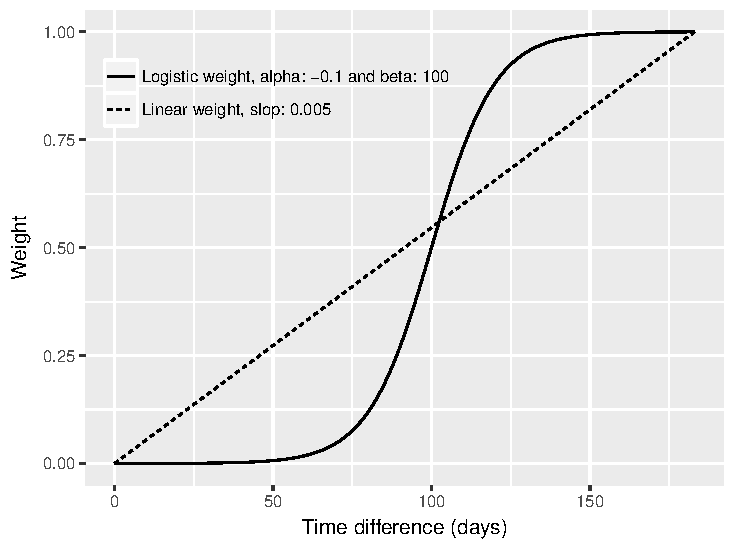
\includegraphics[width=2.7952755in]{applying_twdtw_files/figure-latex/logist-time-weight-1} 

}

\caption{Logistic time-weight function \code{logisticWeight} with steepness \code{alpha=-0.1} and midpoint \code{beta=100}. The $x$ axis shows the absolute difference between two dates in days and the $y$ axis shows the time-weight \citep{Maus:2016}.}\label{fig:logist-time-weight}
\end{figure}
\end{CodeChunk}

\subsection{Visualising the result of the TWDTW
algorithm}\label{visualising-the-result-of-the-twdtw-algorithm}

\pkg{dtwSat} provides five ways to visualise objects of class
\code{twdtwMatches} through the plot types: \code{matches},
\code{alignments}, \code{classification}, \code{path}, and \code{cost}.
The plot type \code{matches} shows the matching points of the patterns
in the long-term time series; the plot type \code{alignments} shows the
alignments and dissimilarity measures; the plot type \code{path} shows
the low cost paths in the TWDTW cost matrix; and the plot type
\code{cost} allows the visualisation of the cost matrices (local cost,
accumulated cost, and time cost); and the plot type
\code{classification} shows the classification of the long-term time
series based on the TWDTW analysis. The plot methods for class
\code{twdtwMatches} return a \code{ggplot} object, so that users can
further manipulate the result using the \pkg{ggplot2} package. For more
details on visualisation functions, please refer to the \pkg{dtwSat}
documentation in the CRAN \citep{Maus:2015a}.

We now describe the plot types \code{matches} and \code{alignments}. The
code bellow shows how to visualise the matching points of the four best
matches of ``soybean'' pattern in the long-term time series, cf.
\autoref{fig:twdtw-matches}.

\begin{CodeChunk}
\begin{CodeInput}
plot(matches, type="matches", patterns.labels="Soybean", k=4)
\end{CodeInput}
\begin{figure}[!h]

{\centering 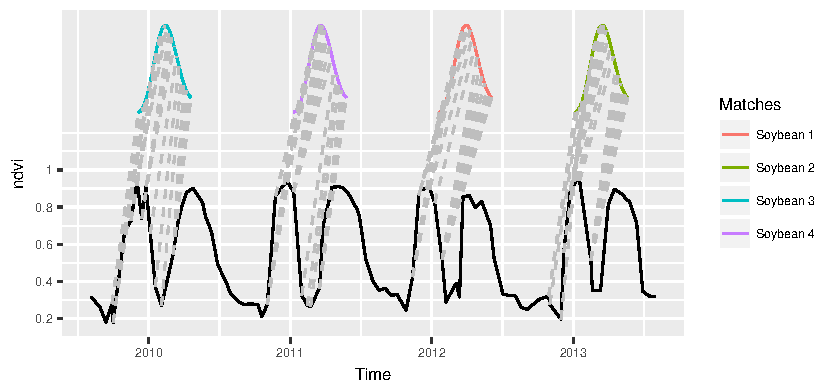
\includegraphics{applying_twdtw_files/figure-latex/twdtw-matches-1} 

}

\caption[The four best matches of the "soybean" pattern in the time series using a logistic time-weight]{The four best matches of the "soybean" pattern in the time series using a logistic time-weight. The solid black line is the long-term time series; the coloured lines are the temporal patterns; and the grey dashed lines are the respective matching points.}\label{fig:twdtw-matches}
\end{figure}
\end{CodeChunk}

The next example uses the plot type \code{alignments} to show the
alignments of the temporal patterns (see
\autoref{fig:alignments-all-patterns}). We set the threshold for the
dissimilarity measure to be lower than \(3.0\). This plot displays the
different subintervals of the long-term time series that have alignments
whose dissimilarity is less than the specified threshold.

\begin{CodeChunk}
\begin{CodeInput}
plot(matches, type="alignments", attr = "evi", threshold = 3.0)
\end{CodeInput}
\begin{figure}[!h]

{\centering 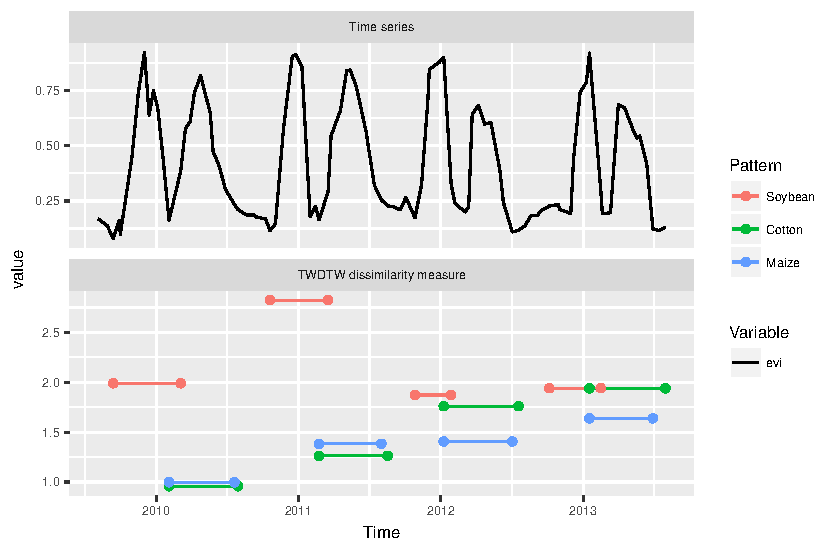
\includegraphics{applying_twdtw_files/figure-latex/alignments-all-patterns-1} 

}

\caption[Alignments and dissimilarity measures of the patterns "soybean", "cotton", and "maize" to the subintervals of the long-term time series using a logistic time-weight]{Alignments and dissimilarity measures of the patterns "soybean", "cotton", and "maize" to the subintervals of the long-term time series using a logistic time-weight. The solid black line is the EVI time series, and the coloured lines are the alignments of the patterns that have dissimilarity measure lower than three.}\label{fig:alignments-all-patterns}
\end{figure}
\end{CodeChunk}

\autoref{fig:alignments-all-patterns} shows the alignments of each
pattern over the long-term time series, note that we can rank the
alignments by their TWDTW dissimilarity, i.e.~alignments overlapping the
same period usually have distinct dissimilarity, which can be used to
rank them. In the figure we can see that maize (blue lines) and cotton
(green lines) overlap approximately the same time periods, however, they
have distinct dissimilarity measures, and therefore, can be ranked.
Observing the time period from January 2010 to July 2010, both soybean,
maize, and cotton have at least one overlapping alignment, however in
this case the cotton pattern matches better to the interval because its
dissimilarity is lower than the others.

\subsection{Classifying the long-term time
series}\label{classifying-the-long-term-time-series}

Using the matches and their associated dissimilarity measures, we can
classify the subintervals of the long-term time series using
\code{twdtwClassify}. To do this, we need to define a period for
classification and the minimum overlap between the period and the
alignments that intersect with it. For each interval,
\code{twdtwClassify} will select the alignment that has the lowest TWDTW
dissimilarity taking into account the minimum overlap condition. For
example, in Figure 7 the interval from 1 September 1012 to 28 February
2013 has three overlapping alignments, maize in blue, cotton in green,
and soybean in red. Without a minimum overlap the function
\code{twdtwClassify} would classify this interval as maize, which has
the lowest dissimilarity in the period. However, if we set a minimum
overlap of 50\%, the function \code{twdtwClassify} classifies the
interval as soybean, which is the only class whose alignment overlaps
the interval during more than 50\% of the time. The interval of
classification are usually defined according to the phenological cycles
or the agricultural calendar of the region. The classification interval
can also be irregular, for details see the argument \code{breaks} in
\code{?twdtwClassify}

In the example bellow we classify each period of 6 months from September
2009 to September 2013; we set a minimum overlap of 50\% between the
alignment and the classification period. This means that at least 50\%
of the alignment has to be contained inside of the classification
period. We also use the plot type \code{classification} to show the
classified subintervals of the long-term time series.

\begin{CodeChunk}
\begin{CodeInput}
ts_classification = twdtwClassify(x = matches, 
  from = as.Date("2009-09-01"), to = as.Date("2013-09-01"), 
  by = "6 month", overlap = 0.5)
plot(ts_classification, type="classification")
\end{CodeInput}
\begin{figure}[!ht]

{\centering 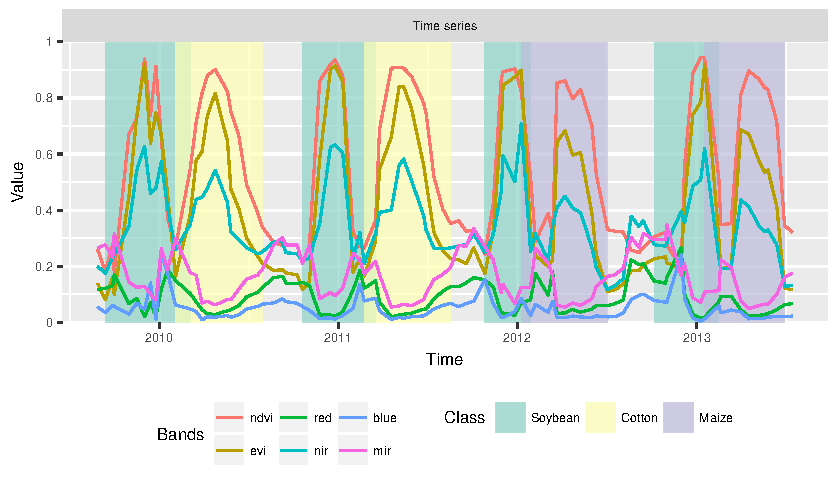
\includegraphics{applying_twdtw_files/figure-latex/time-series-classification-1} 

}

\caption[Classification of each 6 months periods of the time series using results of the TWDTW analysis with logistic time-weight]{Classification of each 6 months periods of the time series using results of the TWDTW analysis with logistic time-weight. The solid lines are the attributes of the time series, the background colours indicate the classification of the periods.}\label{fig:time-series-classification}
\end{figure}
\end{CodeChunk}

By comparing the results of the classified time series in
\autoref{fig:time-series-classification} with the crop cycles in
\autoref{fig:example-timeseries} we see that the algorithm has
classified correctly all the eight subintervals from 2009 to 2013, which
are, respectively: ``Soybean'', ``Cotton'', ``Soybean'', ``Cotton'',
``Soybean'', ``Maize'', ``Soybean'', ``Maize''.

\section{Producing a land cover map}\label{producing-a-land-cover-map}

In this section we present an application of TWDTW for land cover change
analysis using satellite image time series. Our input is a set of
images, each covering the same geographical area at different times.
Each pixel location is then associated to an unclassified satellite
image time series. We assume to have done field work in the area; for
some pixel locations and time periods, we know what is the land cover.
We then will show how to obtain a set of template patterns, based on the
field samples and how to apply these patterns to land cover
classification of the set of images. In the end of this section we show
how to perform land cover change analysis and accuracy assessment.

As an example we classify approximately 5300 km\(^2\) in a tropical
forest region in Mato Grosso, Brazil (\autoref{fig:study-area}). This is
a sequence of 160 images with 999 pixels each for 6 years, from 2007 to
2013. We also have a set of 603 ground truth samples of the following
classes: ``Forest'', ``Cotton-fallow'', ``Soybean-cotton'',
``Soybean-maize'', and ``Soybean-millet''. The satellite images and the
field samples used in the examples come with \pkg{dtwSat} package.

\begin{figure}[!ht]
\begin{center} 
  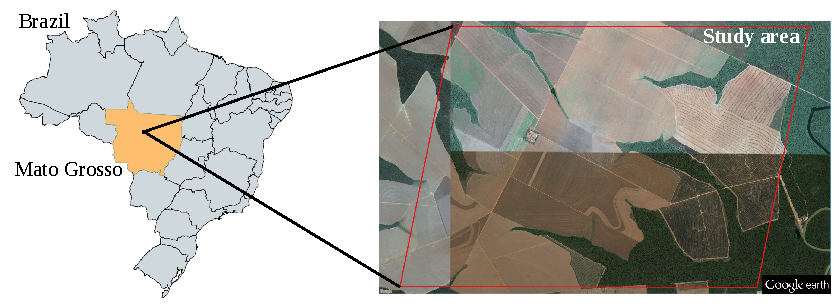
\includegraphics[width=\textwidth]{./study_area.pdf}
\end{center}
\caption{Study area in Mato Grosso, Brazil, shown in a \copyright\ Google Earth image. The area was originally covered by tropical forest that has been removed for agricultural use.}
\label{fig:study-area}
\end{figure}

\subsection{Input data}\label{input-data-1}

The inputs are: \emph{a)} the satellite images for a given geographical
area, organised as a set of georeferenced raster files in GeoTIFF
format, each containing all time steps of a spectral band or index; and
\emph{b)} a set of ground truth samples. The satellite images are
extracted from the MODIS product MOD13Q1 collection 5
\citep{Friedl:2010} and include vegetation indices ``ndvi'', ``evi'',
and original bands ``nir'', ``red'', ``blue'', and ``mir''. This product
has 250 x 250 m spatial resolution and a 16 day maximum-value composite
(MVC) for each pixel location \citep{Friedl:2010}, meaning that one
image can have measurements from different dates. For this reason,
MOD13Q1 also includes the ``day of the year'' (doy) of each pixel as a
layer, which we use to keep the time series consistent with the
measurements.

The data files for the examples that follow are in the \pkg{dtwSat}
installation folder \emph{lucc\_MT/data/}. The \emph{tif} files include
the time series of ``blue'', ``red'', ``nir'', ``mir'', ``evi'',
``ndvi'', and ``doy'' (day of the year); the text file \emph{timeline}
has the dates of the satellite images; the CSV file \emph{samples.csv}
has the \code{longitude}, \code{latitude}, \code{from}, \code{to}, and
\code{label} for each field sample; and the text file
\emph{samples\_projection} contains information about the cartographic
projection of the samples, in the format of coordinate reference system
used by \code{sp::CRS}.

\begin{CodeChunk}
\begin{CodeInput}
data_folder = system.file("lucc_MT/data", package = "dtwSat")
dir(data_folder)
\end{CodeInput}
\begin{CodeOutput}
 [1] "blue.tif"           "doy.tif"            "evi.tif"           
 [4] "mir.tif"            "ndvi.tif"           "nir.tif"           
 [7] "red.tif"            "samples.csv"        "samples_projection"
[10] "timeline"          
\end{CodeOutput}
\end{CodeChunk}

We have stored all the time series for each band in one single file. In
this way, we can use the function \code{raster::brick} to read the
satellite images. The algorithm also works when the time steps for each
band are split in many files. In this case, the user should call the
function \code{raster::stack} with the appropriate parameters. Because
of processing performance, we suggest that interested users group their
images in bricks and follow the procedures given below.

\begin{CodeChunk}
\begin{CodeInput}
blue = brick(paste(data_folder,"blue.tif", sep = "/"))
red  = brick(paste(data_folder,"red.tif", sep = "/"))
nir  = brick(paste(data_folder,"nir.tif", sep = "/"))
mir  = brick(paste(data_folder,"mir.tif", sep = "/"))
evi  = brick(paste(data_folder,"evi.tif", sep = "/"))
ndvi = brick(paste(data_folder,"ndvi.tif", sep = "/"))
day_of_year  = brick(paste(data_folder,"doy.tif", sep = "/"))
dates = scan(paste(data_folder,"timeline", sep = "/"), what = "dates")
\end{CodeInput}
\end{CodeChunk}

We use these data-sets to create a multiple raster time series, which is
used in the next sections for the TWDTW analysis. \pkg{dtwSat} provides
the constructor \code{twdtwRaster} that builds a multi-band satellite
image time series. The inputs of this function are \code{RasterBrick}
objects with the same temporal and spatial extents, and a vector
(\code{timeline}) with the acquisition dates of the images in the format
\code{"YYYY-MM-DD"}. The argument \code{doy} is combined with
\code{timeline} to get the real date of each pixel, independently from
each other. If \code{doy} is not provided then the dates of the pixels
are given by \code{timeline}, i.e.~all pixels in one image will have the
same date. Products from other sensors, such as the Sentinels and
Landsat, usually have all pixels with same date, therefore the argument
\code{doy} is not needed. This function produces an object of class
\code{twdtwRaster} with the time series of multiple satellite bands.

\begin{CodeChunk}
\begin{CodeInput}
raster_timeseries = twdtwRaster(blue, red, nir, mir, evi, ndvi, 
  timeline = dates, doy = day_of_year)
\end{CodeInput}
\end{CodeChunk}

Our second input is a set of ground truth samples in the CSV file
\emph{samples.csv}, which has a total of 603 samples divided in five
classes: 68 ``cotton-fallow'', 138 ``forest'', 79 ``soybean-cotton'',
134 ``soybean-maize'', and 184 ``soybean-millet''. Reading this CSV
file, we get a \code{data.frame} object, with the spatial location
(\code{latitude} and \code{longitude}), starting and ending dates
(\code{from} and \code{to}), and the \code{label} for each sample.

\begin{CodeChunk}
\begin{CodeInput}
field_samples = read.csv(paste(data_folder,"samples.csv", sep = "/"))
head(field_samples, 5)
\end{CodeInput}
\begin{CodeOutput}
  longitude  latitude       from         to         label
1 -55.98819 -12.03646 2011-09-01 2012-09-01 Cotton-fallow
2 -55.99118 -12.04062 2011-09-01 2012-09-01 Cotton-fallow
3 -55.98606 -12.03646 2011-09-01 2012-09-01 Cotton-fallow
4 -55.98562 -12.03437 2011-09-01 2012-09-01 Cotton-fallow
5 -55.98475 -12.03021 2011-09-01 2012-09-01 Cotton-fallow
\end{CodeOutput}
\begin{CodeInput}
table(field_samples[["label"]])
\end{CodeInput}
\begin{CodeOutput}

 Cotton-fallow         Forest Soybean-cotton  Soybean-maize Soybean-millet 
            68            138             79            134            184 
\end{CodeOutput}
\begin{CodeInput}
proj_str = scan(paste(data_folder,"samples_projection", sep = "/"), 
  what = "character")
proj_str
\end{CodeInput}
\begin{CodeOutput}
[1] "+proj=longlat +datum=WGS84 +no_defs +ellps=WGS84 +towgs84=0,0,0"
\end{CodeOutput}
\end{CodeChunk}

\subsection{Assessing the separability of temporal
patterns}\label{assessing-the-separability-of-temporal-patterns}

The classification is highly dependent on the quality of the temporal
patterns. Therefore, it is useful to perform an analysis to assess the
separability of the temporal pattern. Ideally, one would need patterns
that, when applied to the set of unknown time series, produce consistent
results (see the guidelines for single time series analysis in
\autoref{classifying-a-time-series}). For this reason, before performing
the land cover mapping, we perform a cross validation step. In this way,
the users would assess the separability of their patterns before
classifying a large data set.

In the next example we use the function \code{getTimeSeries} to extract
the time series of each field sample from our raster time series. The
arguments of the function are a set of raster time series, a
\code{data.frame} with spatial and temporal information about the fields
samples (as in the object \code{field_samples} given above), and a
\code{proj4string} with the projection information. The projection
should follow the \code{sp::CRS} format. The result is an object of
class \code{twdtwTimeSeries} with one time series for each field sample.

\begin{CodeChunk}
\begin{CodeInput}
field_samples_ts = getTimeSeries(raster_timeseries, 
  y = field_samples, proj4string = proj_str)
field_samples_ts
\end{CodeInput}
\begin{CodeOutput}
An object of class "twdtwTimeSeries"
Slot "timeseries" length: 603 
Slot "labels": [1] "Cotton-fallow" "Cotton-fallow" "Cotton-fallow"
\end{CodeOutput}
\end{CodeChunk}

To perform the cross-validation we use the function
\code{twdtwCrossValidate}. This function splits the sample time series
into training and validation sets using stratified sampling with a
simple random sampling within each stratum, for details see
\code{?caret::createDataPartition}. The function uses the training
samples to create the temporal patterns and then classifies the
remaining validation samples using \code{twdtwApply}. The results of the
classification are used in the accuracy calculation.

A Generalized Additive Model (GAM) {[}Hastie:1986,Wood:2011{]} generates
the smoothed temporal patterns based on the training samples. We use the
GAM because of its flexibility for non-parametric fits, with less
rigorous assumptions on the relationship between response and predictor.
This potentially provides better fit to satellite data than purely
parametric models, due to the data's inter- and intra-annual
variability.

In the next example we set the arguments \code{times=100} and
\code{p=0.1}, which creates 100 different data partitions, each with
10\% of the samples for training and 90\% for validation. The other
arguments of this function are: the logistic weight function with
steepness \texttt{-0.1} and midpoint \texttt{50} to \code{weight.fun};
the frequency of the temporal patterns to 8 days \code{freq=8}, and GAM
smoothing formula to \code{formula = y ~ s(x)}, where function \code{s}
sets up a spline model, with \code{x} the time and \code{y} a satellite
band (for details see \code{?mgcv::gam} and \code{?mgcv::s}). The output
is an object of class \code{twdtwCrossValidation} which includes the
accuracy for each data partition. The object has two slots, the first
called \code{partitions} has the index of the samples used for training,
the second called \code{accuracy} has overall accuracy, user's accuracy,
producer's accuracy, error matrix, and the data used in the calculation,
i.e.~reference classes, predicted classes, and TWDTW distance measure.

\begin{CodeChunk}
\begin{CodeInput}
set.seed(1)
log_fun = logisticWeight(alpha=-0.1, beta=50) 
cross_validation = twdtwCrossValidate(field_samples_ts, times=100, p=0.1, 
  freq = 8, formula = y ~ s(x, bs="cc"), weight.fun = log_fun)
\end{CodeInput}
\end{CodeChunk}

\autoref{fig:plot-accuracy} and \autoref{tab:cross-validation} show the
95\% confidence interval of the mean for user's and producer's accuracy
derived from the hundred-fold cross-validation analysis. The user's
accuracy gives the confidence and the producer's accuracy gives the
sensitivity of the method for each class. In our analysis all classes
had high user's and producer's accuracy, meaning that TWDTW has high
confidence and sensitivity for the classes included in the analysis. The
cross-validation results show that if we randomly select 10\% of our
sampels to create temporal patterns we can get an overall accuracy of at
least 97\% in the classification of the remaining samples with 95\%
confidence level.

\begin{CodeChunk}
\begin{figure}[!ht]

{\centering 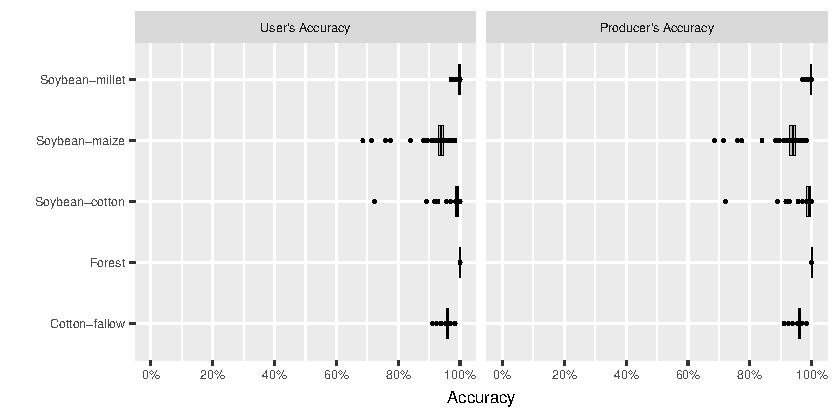
\includegraphics{applying_twdtw_files/figure-latex/plot-accuracy-1} 

}

\caption[User's and producer's accuracy of the TWDTW cross-validation using 100 resampling-with-replacement]{User's and producer's accuracy of the TWDTW cross-validation using 100 resampling-with-replacement. The plot shows the 95\% confidence interval of the mean.}\label{fig:plot-accuracy}
\end{figure}
\end{CodeChunk}

\begin{table}[!ht]
\centering
\begin{tabular}{rlllllllll}
  \hline
   & \multicolumn{3}{c}{User's} & \multicolumn{3}{c}{Producer's} & \multicolumn{3}{c}{Overall}\\
\multicolumn{1}{c}{Class} & \multicolumn{1}{c}{$\mu$} & \multicolumn{1}{c}{$\sigma$} & \multicolumn{1}{c}{ci*} & \multicolumn{1}{c}{$\mu$} & \multicolumn{1}{c}{$\sigma$} & \multicolumn{1}{c}{ci*} & \multicolumn{1}{c}{$\mu$} & \multicolumn{1}{c}{$\sigma$} & \multicolumn{1}{c}{ci*}\\
 \hline
Cotton-fallow & 0.96 & (0.01) & [0.96-0.96] & 1.00 & (0.00) & [1.00-1.00] & 0.98 & (0.02) & [0.97-0.98] \\ 
  Forest & 1.00 & (0.00) & [1.00-1.00] & 1.00 & (0.00) & [1.00-1.00] &  &  &  \\ 
  Soybean-cotton & 0.99 & (0.03) & [0.98-1.00] & 0.89 & (0.02) & [0.89-0.89] &  &  &  \\ 
  Soybean-maize & 0.94 & (0.05) & [0.93-0.95] & 1.00 & (0.01) & [1.00-1.00] &  &  &  \\ 
  Soybean-millet & 1.00 & (0.01) & [1.00-1.00] & 0.98 & (0.05) & [0.97-0.99] &  &  &  \\ 
   \hline 
\multicolumn{10}{l}{* 95\% confidence interval.}
\end{tabular}
\caption{\label{tab:cross-validation} User's and producer's accuracy of the TWDTW cross-validation using 100 resampling-with-replacement. The table shows the standard deviation ($\sigma$) and the 95\% confidence interval (ci) of the mean ($\mu$).'} 
\end{table}

\subsection{Creating temporal
patterns}\label{creating-temporal-patterns}

In the last section we observed that the land cover classes based on our
samples are separable using the TWDTW algorithm with high confidence
level. Now we randomly select 10\% of our samples for training and keep
the remaining 90\% for validation. The first set of samples are used to
create temporal patterns and classify the raster time series, and the
second set of samples to assess the final maps. Ideally we would need a
second independent set of samples to assess the map, but it would be
very difficult to identify different crops without field work.
Therefore, we use the same samples used in the cross-validation
(\autoref{assessing-the-separability-of-temporal-patterns}).

\begin{CodeChunk}
\begin{CodeInput}
library(caret) 
set.seed(1)
I = unlist(createDataPartition(field_samples[,"label"], p = 0.1))
training_ts = subset(field_samples_ts, I)
validation_samples = field_samples[-I,]
\end{CodeInput}
\end{CodeChunk}

We use the function \code{createPatterns} to produce the temporal
patterns based on the training samples. For that, we need to set the
desired temporal frequency of the patterns and the smoothing function
for the GAM model. In the example below, we set \code{freq=8} to get
temporal patterns with a frequency of 8 days, and the GAM smoothing
formula \code{formula = y ~ s(x)}, such as in
\autoref{assessing-the-separability-of-temporal-patterns}).

\begin{CodeChunk}
\begin{CodeInput}
temporal_patterns = 
  createPatterns(training_ts, freq = 8, formula = y ~ s(x))
\end{CodeInput}
\end{CodeChunk}

The result of the function \code{createPatterns} is an object of the
class \code{twdtwTimeSeries}. We use the plot method
\code{type="patterns"} to show the results of the \code{createPatterns}
in \autoref{fig:temporal-patterns}.

\begin{CodeChunk}
\begin{CodeInput}
plot(temporal_patterns, type = "patterns") + 
  theme(legend.position = c(.8,.25))
\end{CodeInput}
\begin{figure}[!h]

{\centering 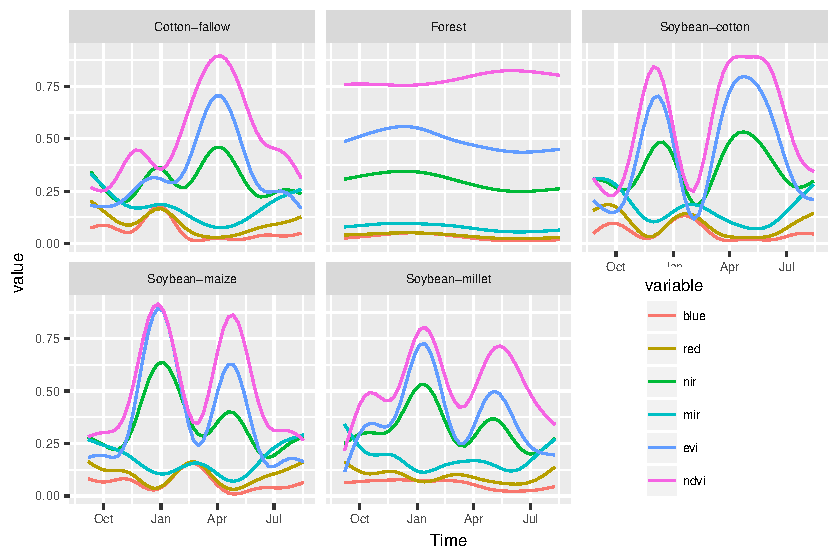
\includegraphics{applying_twdtw_files/figure-latex/temporal-patterns-1} 

}

\caption[Temporal patterns of Forest, Cotton-fallow, Soybean-cotton, Soybean-maize, and Soybean-millet based on the ground truth samples]{Temporal patterns of Forest, Cotton-fallow, Soybean-cotton, Soybean-maize, and Soybean-millet based on the ground truth samples.}\label{fig:temporal-patterns}
\end{figure}
\end{CodeChunk}

Our method is not restricted to cases where the temporal patterns are
obtained from the set of images, such as in the example above. Once can
also use patterns from a different set of images or defined in other
studies, as long as these temporal patterns stand for the study area and
their bands match the bands in the unclassified images.

\subsection{Classifying the image time
series}\label{classifying-the-image-time-series}

After obtaining a consistent set of temporal patterns, we use the
function \code{twdtwApply} to run the TWDTW analysis for each pixel
location in the raster time series. The input raster time series in the
object \code{twdtwRaster} should be longer or have approximatly the same
length as the temporal patterns. This function retrieves an object of
class \code{twdtwRaster} with the TWDTW dissimilarity measure of the
temporal patterns for each time period. The arguments \code{overwrite}
and \code{format} are passed to \code{raster::writeRaster}. The
arguments \code{weight.fun} and \code{overlap} are described in
\autoref{classifying-a-time-series}. Here we set the parameters of the
time weight (logistic function) base on our the experience about the
phenological cycle of the vegetation in the study area. In the next
example, we classify the raster time series using the temporal patterns
in \code{temporal_patterns} obtained as described above. The result is a
\code{twdtwRaster} with five layers; each layer contains the TWDTW
dissimilarity measure for one temporal pattern over time. We use the
plot type \code{distance} to illustrate the TWDTW dissimilarity for each
temporal pattern in 2008, cf. \autoref{fig:plot-dissmilarity2008}.

\begin{CodeChunk}
\begin{CodeInput}
log_fun = logisticWeight(alpha=-0.1, beta=50) 
twdtw_dist = twdtwApply(x = raster_timeseries, y = temporal_patterns, 
  overlap = 0.5, weight.fun = log_fun, overwrite=TRUE, format="GTiff")
\end{CodeInput}
\begin{CodeOutput}
[1] "Procesing chunk 1/1"
\end{CodeOutput}
\end{CodeChunk}

\begin{CodeChunk}
\begin{CodeInput}
plot(x = twdtw_dist, type="distance")
\end{CodeInput}
\begin{figure}[!ht]

{\centering 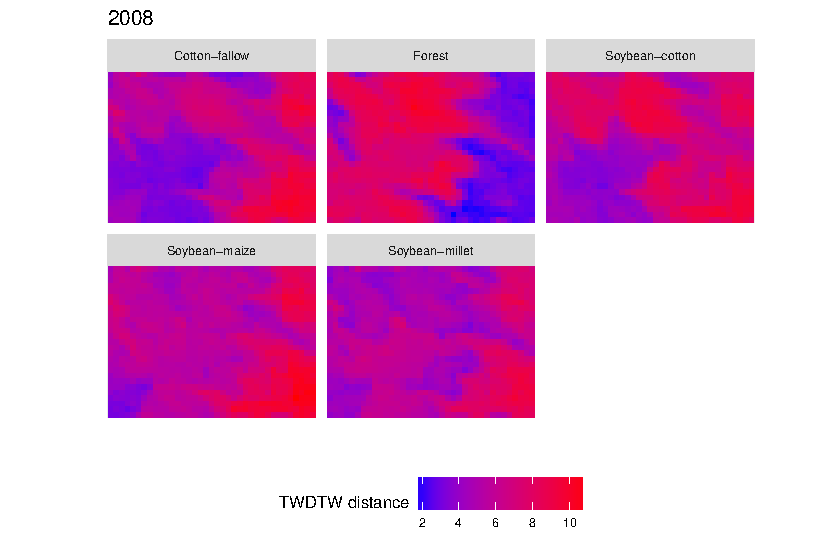
\includegraphics{applying_twdtw_files/figure-latex/plot-dissmilarity2008-1} 

}

\caption[Illustration of the TWDTW dissimilarity from each temporal pattern in 2008]{Illustration of the TWDTW dissimilarity from each temporal pattern in 2008. The blue areas are more similar to the pattern and the red areas are less similar to the pattern.}\label{fig:plot-dissmilarity2008}
\end{figure}
\end{CodeChunk}

The results of the example above can be used to create categorical land
cover maps. The function \code{twdtwClassify} selects the most similar
pattern for each time period and retrieves a \code{twdtwRaster} object
with the time series of land cover maps. The resulting object includes
two layers, the first has the classified categorical maps and the second
has the TWDTW dissimilarity measure.

\begin{CodeChunk}
\begin{CodeInput}
land_cover_maps = twdtwClassify(twdtw_dist, format="GTiff", overwrite=TRUE)
\end{CodeInput}
\end{CodeChunk}

\subsection{Looking at the classification
results}\label{looking-at-the-classification-results}

The classification results can be visualised using the \code{plot}
methods of the class \code{twdtwRaster}, which supports four plot types:
``maps'', ``area'', ``changes'', and ``distance''. The
\code{type="maps"} shows the land cover classification maps for each
period, cf. \autoref{fig:plot-map}.

\begin{CodeChunk}
\begin{CodeInput}
plot(x = land_cover_maps, type = "maps")
\end{CodeInput}
\begin{figure}[!ht]

{\centering 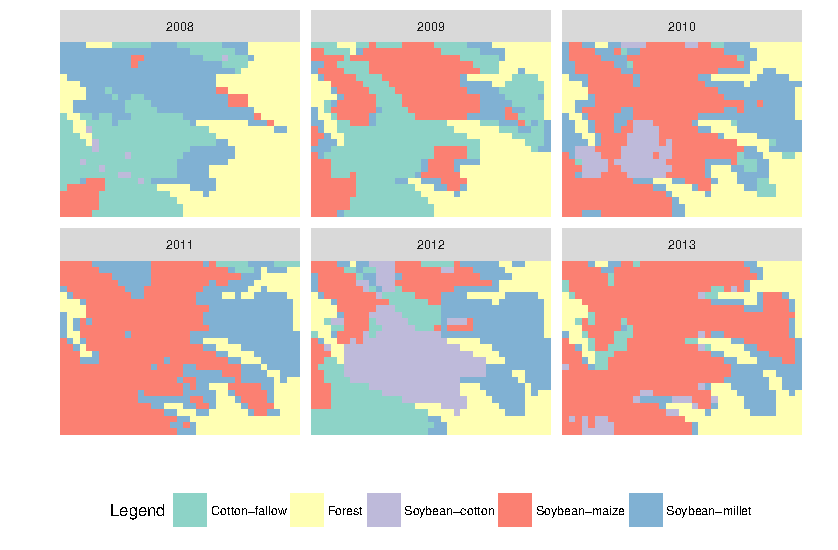
\includegraphics{applying_twdtw_files/figure-latex/plot-map-1} 

}

\caption[Land cover maps for each year from 2008 to 2013]{Land cover maps for each year from 2008 to 2013.}\label{fig:plot-map}
\end{figure}
\end{CodeChunk}

The next example shows the accumulated area for each class over time,
using \code{type="area"}, cf. \autoref{fig:plot-area}.

\begin{CodeChunk}
\begin{CodeInput}
plot(x = land_cover_maps, type = "area")
\end{CodeInput}
\begin{figure}[!ht]

{\centering 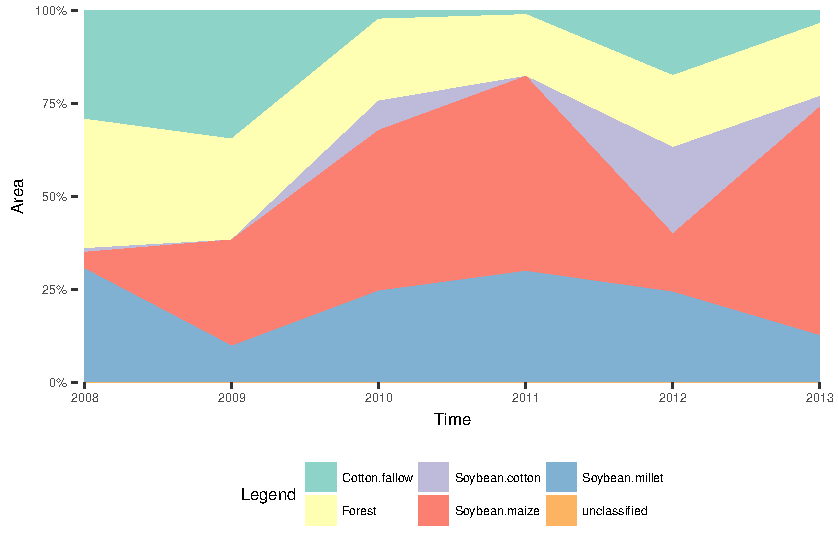
\includegraphics{applying_twdtw_files/figure-latex/plot-area-1} 

}

\caption[Percentage of area for each land cover class from 2008 to 2013]{Percentage of area for each land cover class from 2008 to 2013.}\label{fig:plot-area}
\end{figure}
\end{CodeChunk}

Users can also view the land cover transition for each time period, by
setting \code{type="changes"}. For each land cover class and each
period, the plot shows gains and losses in area from the other classes.
This is the visual equivalent of a land transition matrix, cf.
\autoref{fig:plot-change}.

\begin{CodeChunk}
\begin{CodeInput}
plot(x = land_cover_maps, type = "changes")
\end{CodeInput}
\begin{figure}[!h]

{\centering 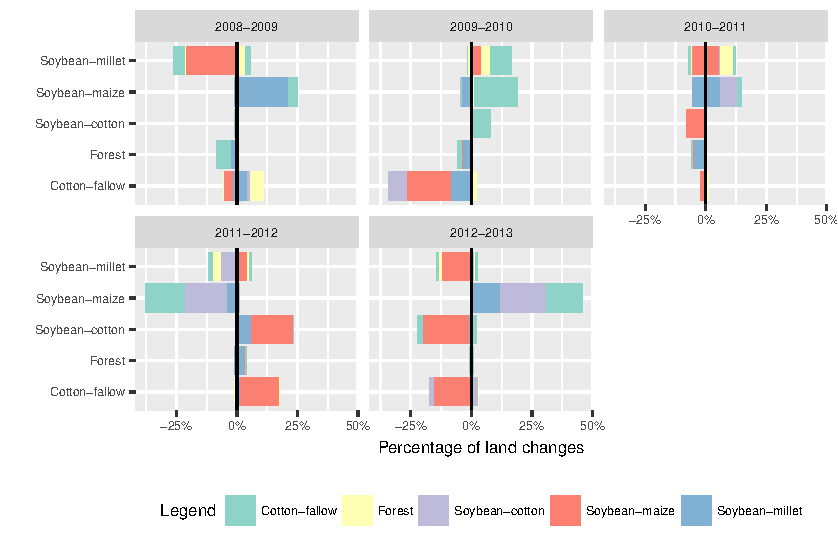
\includegraphics{applying_twdtw_files/figure-latex/plot-change-1} 

}

\caption[Gains and losses in area from the other classes]{Gains and losses in area from the other classes. The $y$ axis shows the actual class; the positive direction of $x$ axis shows the gains and the negative direction of $x$ axis shows the losses of the classes indicated in $y$. The colors indicate from/to which classes the gains/losses belong.}\label{fig:plot-change}
\end{figure}
\end{CodeChunk}

We can also look at the dissimilarity of each classified pixel setting
\code{type="distance"}. This plot can give a measure of the uncertainty
of the classification of each pixel for each time period, cf.
\autoref{fig:plot-dissmilarity}.

\begin{CodeChunk}
\begin{CodeInput}
plot(x = land_cover_maps, type="distance")
\end{CodeInput}
\begin{figure}[!ht]

{\centering 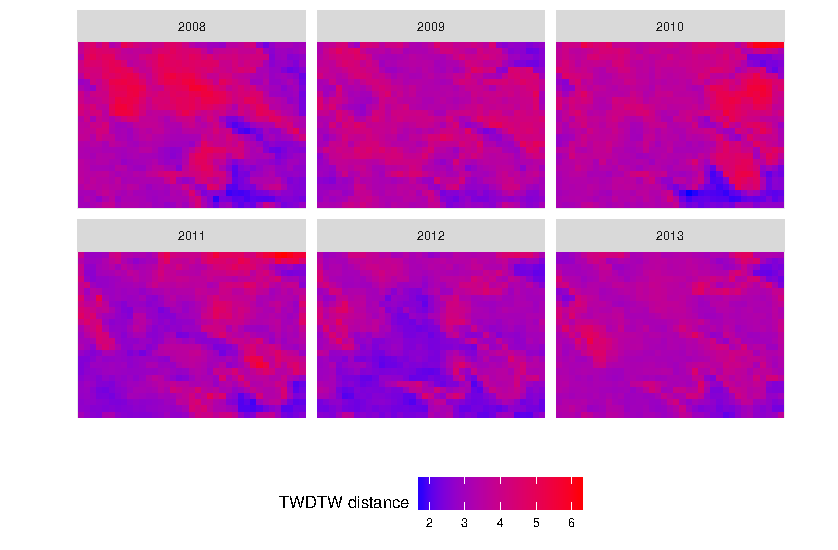
\includegraphics{applying_twdtw_files/figure-latex/plot-dissmilarity-1} 

}

\caption[TWDTW dissimilarity measure for each pixel over each classified period]{TWDTW dissimilarity measure for each pixel over each classified period. The blue areas have high confidence and the red areas have low confidence in the classification.}\label{fig:plot-dissmilarity}
\end{figure}
\end{CodeChunk}

\subsection{Assessing classification
accuracy}\label{assessing-classification-accuracy}

In this section we show how to assess the classification. \pkg{dtwSat}
provides a function called \code{twdtwAssess}, which computes a set of
accuracy metrics, and adjusted area such as proposed by
\citet{Olofsson:2013} and \citet{Olofsson:2014}. The inputs of this
function are the classified map (an object of class \code{twdtwRaster}),
and a set of samples for validation (an object of class
\code{data.frame} or \code{sp::SpatialPointsDataFrame}). Besides
coordinates, the samples should also have starting dates, ending dates,
and lables compatible with the labels in the map (for details see
\autoref{input-data}). The output of \code{twdtwAssess} is an object of
class \code{twdtwAssessment}, which includes four slots: 1)
\code{accuracyByPeriod} is a list of metrics for each time period,
including overall accuracy, user's accuracy, produce's accuracy, error
matrix (confusion matrix), and adjusted area; 2) \code{accuracySummary}
has the accuracy and adjusted area accumulated over all time periods; 3)
\code{data} is a \code{SpatialPointsDataFrame} with sample ID, period
ID, starting date, ending date, reference label, predicted label, and
TWDTW distance; and 4) \code{map} is a twdtwRaster with the raster maps.
The next example uses \code{twdtwAssess} to compute the accuracy of the
maps (\code{land_cover_maps}) using the validation samples
(\code{validation_samples}) with a 95\% confidence level.

\begin{CodeChunk}
\begin{CodeInput}
maps_assessment = twdtwAssess(land_cover_maps, y = validation_samples, 
  proj4string = proj_str, conf.int=.95)
\end{CodeInput}
\end{CodeChunk}

The results of the assessment in \autoref{tab:map-error-matrix},
\ref{tab:map-accuracy}, and \ref{tab:map-adjusted-area} are accumulated
over the whole time period, i.e.~the total mapped area is equal to the
surface area times the number of maps. It is possible to assess and
visualise each period independently from each other. However, our
samples are irregularly distributed over time and some classes do not
have samples in all time period, which limits the analysis of each time
period independently from each other.

\begin{table}[!ht]
\centering
\begin{tabular}{rrrrrrrrr}
  \hline
  &\multicolumn{5}{c}{Reference class}&&\\
\multicolumn{1}{c}{Map class} & \rotatebox[origin=l]{90}{Cotton-fallow} & \rotatebox[origin=l]{90}{Forest} & \rotatebox[origin=l]{90}{Soybean-cotton} & \rotatebox[origin=l]{90}{Soybean-maize} & \rotatebox[origin=l]{90}{Soybean-millet} & Total & Area & w\\
 \hline
Cotton-fallow & 61 & 0 & 3 & 0 & 0 & 64 & 47600561 & 0.148 \\ 
  Forest & 0 & 124 & 0 & 0 & 0 & 124 & 74754883 & 0.232 \\ 
  Soybean-cotton & 0 & 0 & 62 & 0 & 0 & 62 & 18782634 & 0.058 \\ 
  Soybean-maize & 0 & 0 & 6 & 120 & 0 & 126 & 110173564 & 0.343 \\ 
  Soybean-millet & 0 & 0 & 0 & 0 & 165 & 165 & 70354380 & 0.219 \\ 
  Total & 61 & 124 & 71 & 120 & 165 & 541 & 321666022 & 1.000 \\ 
   \hline
\end{tabular}
\caption{\label{tab:map-error-matrix}Error matrix of the map classification based on TWDTW analysis. The area is in the map unit, in this case $m^2$. $w$ is the proportion of area mapped for each class.} 
\end{table}

As we can see in \autoref{tab:map-error-matrix} only nine samples were
misclassified, all of them from the reference class ``Soybean-cotton''.
From these samples six were classified as ``Soybean-maize'', and three
as ``Cotton-fallow''. As we see in \autoref{tab:map-accuracy} the only
class with producer's accuracy lower than \(100\%\) was
``Soybean-cotton'', reaching \(72\%\) with high uncertainty
(\(\pm13\%\)). The user's accuracy for all classes was higer than
\(95\%\), with maximun uncertainty of \(\pm5\%\). To visualise the
misclassified samples on top of the maps we can use the plot
\code{type="map"} for objects of class \code{twdtwAssessment}, such that
\texttt{plot(x\ =\ maps\_assessment,\ type="map",\ samples="incorrect")}.
The user can also set the argument \code{samples} to see correctly
classified samples \code{samples="correct"}, or to see all samples
\code{samples="all"}.

The \autoref{fig:plot-map-incorrect-samples} shows that the
misclassified samples are all in the map from 2012. The six samples of
``Soybean-cotton'' classified as ``Soybean-maize'' are within a big area
of ``Soybean-maize'' and the three samples of ``Soybean-cotton''
classified as ``Cotton-fallow'' are near the border between this two
classes. This errors might be related to the mixture of different
classes in the same pixel.

\begin{CodeChunk}
\begin{figure}[!ht]

{\centering 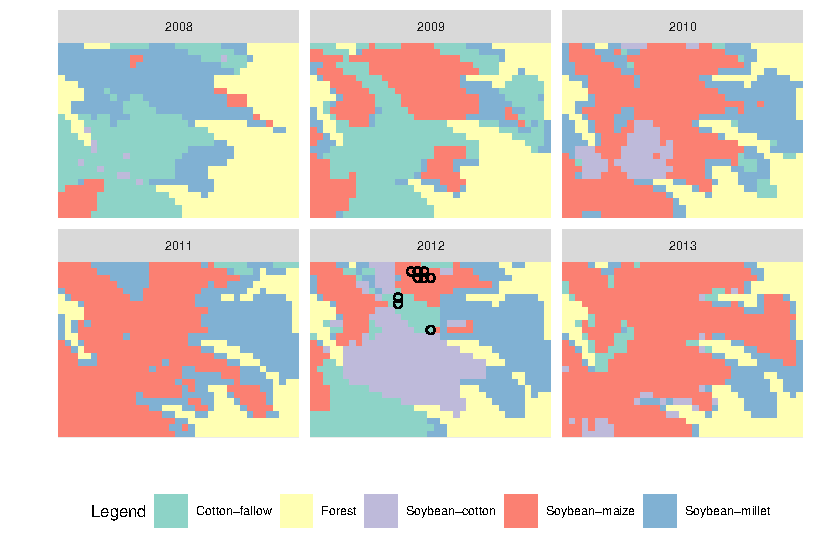
\includegraphics{applying_twdtw_files/figure-latex/plot-map-incorrect-samples-1} 

}

\caption[Incorrect classified samples]{Incorrect classified samples.}\label{fig:plot-map-incorrect-samples}
\end{figure}
\end{CodeChunk}

\begin{table}[!ht]
\centering
\begin{tabular}{rlllllllll}
  \hline
  &\multicolumn{5}{c}{Reference class}&&&&\\
\multicolumn{1}{c}{Map class} & \rotatebox[origin=l]{90}{Cotton-fallow} & \rotatebox[origin=l]{90}{Forest} & \rotatebox[origin=l]{90}{Soybean-cotton} & \rotatebox[origin=l]{90}{Soybean-maize} & \rotatebox[origin=l]{90}{Soybean-millet} & Total & User's* & Producers's* & Overall*\\
 \hline
Cotton-fallow & 0.14 & 0.00 & 0.00 & 0.00 & 0.00 & 0.14 & 0.95$\pm$0.05 & 1.00$\pm$0.00 & 0.98$\pm$0.01 \\ 
  Forest & 0.00 & 0.23 & 0.00 & 0.00 & 0.00 & 0.23 & 1.00$\pm$0.00 & 1.00$\pm$0.00 &  \\ 
  Soybean-cotton & 0.01 & 0.00 & 0.06 & 0.02 & 0.00 & 0.08 & 1.00$\pm$0.00 & 0.72$\pm$0.13 &  \\ 
  Soybean-maize & 0.00 & 0.00 & 0.00 & 0.33 & 0.00 & 0.33 & 0.95$\pm$0.04 & 1.00$\pm$0.00 &  \\ 
  Soybean-millet & 0.00 & 0.00 & 0.00 & 0.00 & 0.22 & 0.22 & 1.00$\pm$0.00 & 1.00$\pm$0.00 &  \\ 
  Total & 0.15 & 0.23 & 0.06 & 0.34 & 0.22 & 1.00 &  &  &  \\ 
   \hline 
\multicolumn{9}{l}{* 95\% confidence interval.}
\end{tabular}
\caption{\label{tab:map-accuracy}Accuracy and error matrix in proportion of area of the classified map.} 
\end{table}

In \autoref{tab:map-adjusted-area} we can see the mapped and the
adjusted area. This is the accumulated area over the whole period,
i.e.~the sum of all maps from 2008 to 2013. As the ``Forest'' and
``Soybean-millet'' did not have omission (\(100\%\) producer's accuracy)
or comission (\(100\%\) user's accuracy) erros, we immediately see that
their mapped area is equal to their adjusted area
(\autoref{tab:map-adjusted-area}). To help the analysis of the other
classes we use the plot \code{type="area"} for class
\code{twdtwAssessment}, such that
\texttt{plot(x\ =\ maps\_assessment,\ type="area",\ perc=FALSE)}.
\autoref{fig:plot-area-and-uncertainty} shows the accumulated area
mapped and adjusted for all classes. In this figure we see that our
method overestimated the area of ``Soybean-maize'', i.e.~the mapped area
(\(110173564\;m^2\)) is bigger than the adjusted area
(\(104927204\;m^2\)) plus the confidence interval \(4113071\;m^2\).
Meanwhile we underestimated the area of ``Soybean-cotton'', i.e.~its
mapped area (\(18782634\;m^2\)) is smaller than the adjusted area
(\(26260270\;m^2\)) plus the confidence interval (\(4805205\;m^2\)). The
mapped area of ``Cotton-fallow'' (\(47600561\;m^2\)) is within the
confidence interval of the adjusted area (\(45369285\pm2484480\;m^2\)).
To improve the accuracy assessment and area estimations the field
samples should be better distributed over time, which would also allow
for better land cover changes assessment.

\begin{table}[!ht]
\centering
\begin{tabular}{rlll}
  \hline
  \multicolumn{1}{c}{Class} & Mapped area & Adjusted area & Margin of error*\\
 \hline
Cotton-fallow & 47600561 & 45369285 & $\pm$2484480 \\ 
  Forest & 74754883 & 74754883 & $\pm$0 \\ 
  Soybean-cotton & 18782634 & 26260270 & $\pm$4805205 \\ 
  Soybean-maize & 110173564 & 104927204 & $\pm$4113071 \\ 
  Soybean-millet & 70354380 & 70354380 & $\pm$0 \\ 
   \hline 
\multicolumn{3}{l}{* 95\% confidence interval.}
\end{tabular}
\caption{\label{tab:map-adjusted-area}Mapped and adjusted, accumulated over the whole period, i.e. the sum from the sum of the maps from 2008 to 2013. The area is in the map unit, in this case $m^2$.} 
\end{table}

\begin{CodeChunk}
\begin{figure}[!ht]

{\centering 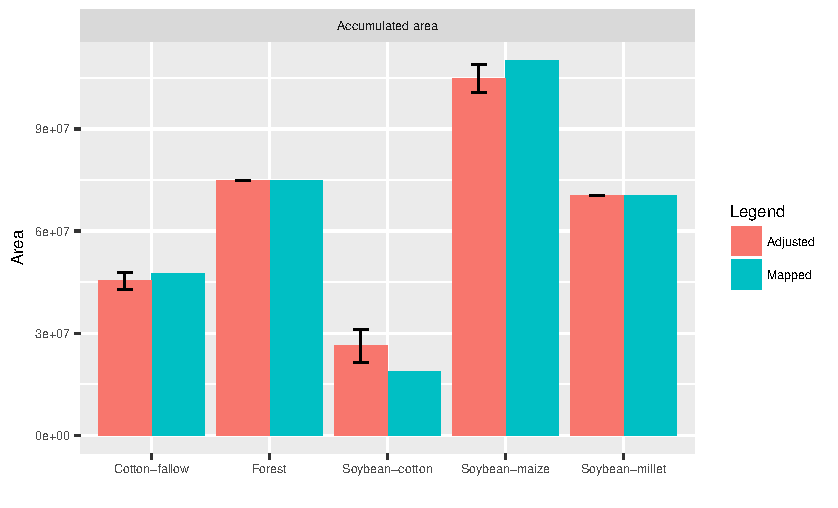
\includegraphics{applying_twdtw_files/figure-latex/plot-area-and-uncertainty-1} 

}

\caption[Mapped and adjusted, accumulated over the whole period, i.e]{Mapped and adjusted, accumulated over the whole period, i.e. the sum from the sum of the maps from 2008 to 2013. The area is in the map unit, in this case $m^2$.}\label{fig:plot-area-and-uncertainty}
\end{figure}
\end{CodeChunk}

\section{Conclusions and Discussion}\label{conclusions-and-discussion}

The overall accuracy of the classification with a 95\% confidence level
is within 97\% and 99\%. With same confidence level, user's and
producer's accuracy are between 90\% and 100\% for all classes, except
for ``Soybean-cotton'', which has wide confidence interval for user's
accuracy, between 59\% and 85\%. A small sample size will likely have
large confidence intervals \citep{Foody:2009}, therefore, this analysis
could be improved by increasing the number of ``Soybean-cotton''
samples. In addition, our access to field information is limited to a
set of samples irregularly distributed over time, which are not enough
to assess each mapped period independently from each other.
Nevertheless, the results of the accuracy assessment show that the TWDTW
has great potential to classify different crop types.

DTW based approaches have achieved good results for land cover
classification \citep{Petitjean:2012, Maus:2016}, however, a reduced
number of points in the time series will negatively impact the accuracy.
Remotely sensed images often present noise and poor coverage due to
clouds, aerosol load, surface directional effects, and sensor problems.
This leads to large amount of gaps in satellite image time series.
Therefore, methods that deal with irregular temporal sampling,
i.e.~irregular sampling intervals, have great potential to fully exploit
the available satellite images archive. DTW is known to be one of the
most robust methods for irregular time series
\citep{Keogh:2005, Tormene:2009}. It was successfully applied for
satellite time series clustering using FORMOSAT-2 \citep{Petitjean:2012}
and using MODIS \citep{Maus:2016}. \citet{Petitjean:2012}, for example,
showed that clustering based on DTW is consistent even when there are
several images missing per year because of cloud cover. However, the
effect of a reduced number of samples in the time needs to be better
evaluated in order to point out the limiting gap size for satellite
image time series analysis using DTW based methods.

The DTW approaches will search for the matches of a temporal pattern,
therefore the number of points in the time series should represent the
phenological cycles of different land cover types. The number of
available observations might be a limitation for sensors with lower
temporal resolution, such as Landsat. We believe that this limitation
could be addressed, for example, by combining TWDTW analysis with
pixel-based compositing techniques \citep{Griffiths:2013, White:2014}.
These approaches have become more popular with the opening of the USGS
Landsat archive and could be used to increase the availability of
gap-free time series \citep{Gomez:2016}.

\pkg{dtwSat} provides a dissimilarity measure in the n-dimensional
space, allowing multispectral satellite image time series analysis. Our
experience using MODIS data sets has shown that n-dimensional analysis,
i.e.~using RED, NIR, NDVI, EVI, and NDVI, increases the separability
among classes when compared to single band analysis, for example using
only EVI or NDVI. Further studies on multispectral data using TWDTW
analysis will help to optimize the selection of bands.

The main goal of \pkg{dtwSat} package is to make TWDTW accessible for
researchers. The package supports the full cycle of land cover
classification using image time series, ranging from selecting temporal
patterns to visualising and assessing the results. The current version
of the \pkg{dtwSat} package provides a pixel-based time series
classification method. We envisage that future versions of the package
could include local neighborhoods to reduce border effects and improve
classification homogeneity.

The \pkg{dtwSat} package provides two in-built functions for linear and
logistic time weight. In the current version of the package the
parameters of the weight functions are set manually to the same value
for all land cover classes. Future versions could include methods to
search for the best parameters for each land cover class using field
data.

Nowadays, there are large open archives of Earth Observation data, but
few open source methods for analysing them. With this motivation, this
paper provides guidance on how to use the Time-Weighed Dynamic Time
Warping (TWDTW) method for remote sensing applications. As we have
discussed in a companion paper \citep{Maus:2016}, the TWDTW method is
well suited for land cover change analysis of satellite image time
series.

The TWDTW algorithm is computationally intensive and for large areas one
should consider parallel processing. The algorithm is pixel time series
based, i.e.~each time series is processed independently from each other,
and therefore, it can be easily parallelized. To aim for maximum usage
by the scientific community, the \pkg{dtwSat} package described in this
paper works with well-known \proglang{R} data classes such as provided
by \pkg{raster}, which offers the option to work with raster data sets
stored on disk that are too large to be loaded into memory (RAM) at once
\citep{Hijmans:2015}. We are planning improvements, so that \pkg{dtwSat}
can also be combined with array databases, such as SciDB
\citep{Stonebraker:2013}. We believe that combining array databases with
image time series analysis software such as presented here is one way
forward to scaling the process of information extracting from very large
Earth Observation data.

\section*{Acknowledgments}

Victor Maus has been supported by the Institute for Geoinformatics,
University of Münster (Germany), and by the Earth System Science Center,
National Institute for Space Research (Brazil). Gilberto Camara's term
as Brazil Chair at IFGI has been supported by CAPES (grant
23038.007569/2012-16). Gilberto's work is also supported by FAPESP
e-science program (grant 2014-08398-6) and CNPq (grant 312151/2014-4).

\bibliography{references.bib}


\end{document}

